%%%% ijcai18.tex

\typeout{Galaxy Network Embedding: A Hierarchical Community Structure Preserving Approach}

% These are the instructions for authors for IJCAI-18.
% They are the same as the ones for IJCAI-11 with superficical wording
%   changes only.

\documentclass{article}
\pdfpagewidth=8.5in
\pdfpageheight=11in
% The file ijcai18.sty is the style file for IJCAI-18 (same as ijcai08.sty).
\usepackage{ijcai18}

% Use the postscript times font!
\usepackage{times}
\usepackage{xcolor}
\usepackage{soul}
\usepackage[utf8]{inputenc}
\usepackage[small]{caption}

% wy add
\usepackage{helvet}  %Required
\usepackage{courier}  %Required
\usepackage{url}  %Required
\usepackage{graphicx}  %Required
\usepackage{algorithm}
\usepackage{algorithmicx}
\usepackage[noend]{algpseudocode}
\usepackage{amsmath}
\usepackage{bm}

\usepackage{subfigure}

\usepackage{CJK}
\usepackage{array}
\usepackage{amsthm}
\usepackage{amssymb}

\theoremstyle{definition}
\newtheorem{defn}{Definition}
\newtheorem{lem}{Lemma}


\renewcommand{\algorithmicrequire}{\textbf{Input:}} % Use Input in the format of Algorithm
\renewcommand{\algorithmicensure}{\textbf{Output:}} % Use Output in the format of Algorithm

%TODO PACKAGE, DELETE THEM ALL!!
\usepackage{lipsum}                     % Dummytext
\usepackage{xargs}                      % Use more than one optional parameter in a new commands
%\usepackage[pdftex,dvipsnames]{xcolor}  % Coloured text etc.
% 
\usepackage[colorinlistoftodos,prependcaption,textsize=tiny]{todonotes}
\newcommandx{\unfinished}[2][1=]{\todo[linecolor=red,backgroundcolor=red!25,bordercolor=red,#1]{#2}}
\newcommandx{\change}[2][1=]{\todo[linecolor=blue,backgroundcolor=blue!25,bordercolor=blue,#1]{#2}}
\newcommandx{\info}[2][1=]{\todo[linecolor=OliveGreen,backgroundcolor=OliveGreen!25,bordercolor=OliveGreen,#1]{#2}}
\newcommandx{\improvement}[2][1=]{\todo[linecolor=Plum,backgroundcolor=Plum!25,bordercolor=Plum,#1]{#2}}
\newcommandx{\thiswillnotshow}[2][1=]{\todo[disable,#1]{#2}}
\newcommand{\origin}[1]{{\color{blue}{#1}}}
\newcommand{\new}[1]{{\color{red}{#1}}}


% the following package is optional:
%\usepackage{latexsym} 

% Following comment is from ijcai97-submit.tex:
% The preparation of these files was supported by Schlumberger Palo Alto
% Research, AT\&T Bell Laboratories, and Morgan Kaufmann Publishers.
% Shirley Jowell, of Morgan Kaufmann Publishers, and Peter F.
% Patel-Schneider, of AT\&T Bell Laboratories collaborated on their
% preparation.

% These instructions can be modified and used in other conferences as long
% as credit to the authors and supporting agencies is retained, this notice
% is not changed, and further modification or reuse is not restricted.
% Neither Shirley Jowell nor Peter F. Patel-Schneider can be listed as
% contacts for providing assistance without their prior permission.

% To use for other conferences, change references to files and the
% conference appropriate and use other authors, contacts, publishers, and
% organizations.
% Also change the deadline and address for returning papers and the length and
% page charge instructions.
% Put where the files are available in the appropriate places.

\title{Galaxy Network Embedding: A Hierarchical Community Structure Preserving Approach}

% Single author syntax
\author{Jêröme Lang\\ 
Laboratoire d'Analyse et Modélisation des Systèmes pour l'Aide à la Décision (LAMSADE)  \\
pcchair@ijcai-18.org}

% Multiple author syntax (remove the single-author syntax above and the \iffalse ... \fi here)
\iffalse
\author{
First Author$^1$, 
Second Author$^2$, 
Third Author$^3$, 
\\ 
$^1$ First Affiliation \\
$^2$ Second Affiliation\\
$^3$ Third Affiliation  \\
%
first@email.address,
second@email.address,
third@email.address
}
% If your authors do not fit in the default space, you can increase it 
% by uncommenting the following (adjust the "2.5in" size to make it fit
% properly)
% \setlength\titlebox{2.5in}
\fi

\begin{document}

\maketitle

\begin{abstract}
	Network Embedding is a method to learn the low-dimensional vector representations of nodes under the condition of preserving different kinds of the network properties. Previous works mainly focus on preserving structure information of nodes on a particular resolution, like neighbor information or community information, but cannot preserve the hierarchical community structure which enables the network to be easily analyzed on various resolutions. In this paper, we formulate a constrained optimization problem to describe the hierarchical community structure preserving network embedding. Inspired by the galaxy structure with hierarchy, we propose the Galaxy Network Embedding (GNE) model to solve the sophisticated optimization above effectively. In detail, we present an approach to embed communities into an low dimension spherical surface whose center represents the parent community they belong to. The experiments reveal that the node representations from GNE preserves the hierarchical community structure and shows advantages in several applications such as node multi-class classification and network visualization. The source code of GNE is available online.

\end{abstract}

\section{Introduction}

		Network embedding is an approach to learn the low-dimensional representation of complex network vertices under the condition of preserving different kinds of the structure information of the network. Through the network embedding, many general machine learning methods can be applied for fast and effective vertices classification, clustering and network visualization \cite{bhagat2011node}\cite{yan2007graph}.
		
		Network embedding studies include structure-preserving method \cite{Grover2016node2vec}\cite{Wang2017Community} and property-preserving method \cite{Yang2015Network}\cite{Hu2017Label}. Our paper focuses on preserving structure information. In terms of structure-preserving methods, inspired by skip-gram in word2vec \cite{mikolov2013efficient}, some methods consider the node context and represent a node with its nearby nodes \cite{Perozzi2014DeepWalk}\cite{Grover2016node2vec}. Another line of methods present more explicit optimization to preserve the pair-wise proximity of node, which take full account of the characteristics of network structures \cite{Tang2015LINE}\cite{Cao2015GraRep}\cite{Wang2016Structural}. In addition to preserving the microscopic structure, the community structure, one important mesoscopic description of network structure, is incorporated into network embedding in MNMF, of which the learned embedding space can well reflect the organizational structures and functional components of networks \cite{Wang2017Community}.

		Essentially, these methods mainly focus on preserving neighborhood information, or community structure on a particular scale. 
		Nevertheless, the community structure of a complex network is hierarchical \cite{clauset2006structural}, and even some complex networks are in explicitly hierarchical structure, such as (wordnet) social networks, air transportation networks, and metabolic networks. 
		In the presence of hierarchy, the concept of community structure becomes richer \cite{sales-pardo2007extracting}. For instance, in the chemical network, amino acids constitute proteins, which in turn are composed of basic chemical elements. 
		In a word, the hierarchical community preserving network embedding can provide richer structural information, and make it easier to analyze the network on different resolutions.

		It is challenging to formulate the hierarchical community preserving network embedding. Not only the topology relationship between the nodes of the same layer needs to be considered, but the relationship between different levels needs to be considered. In addition to formulate an effective optimization, designing a model to efficiently solve it is a challenge as well. 

		In this paper, in order to preserve the hierarchical community structure for the networks in explicit hierarchy, we define a constrained optimization problem on network embedding. To the best of our knowledge, two types of relationship should be preserved on the hierarchical community network embedding. The first is local information which preserves the microscopic structure (pairwise node similarity) in the same community at a certain layer. The second is hierarchy information. Horizontally, the nodes in the same community are more similar to each other. Vertically, a community in the deeper level has a greater cohesion degree (E.g. The earth is closer to the moon, farther from the sun). Thus, an optimization extends from GraRep \cite{Cao2015GraRep}, is defined to preserve the pairwise similarity between communities, with constraints on hierarchy horizontally and vertically. 

		In order to solve the sophisticated non-convex optimization with constraints efficiently, we propose the Galaxy Network Embedding Model. The galaxy, another type of systems with hierarchical structure, has two desirable structural characteristics which ensures that the embedding results preserve the essence of hierarchy: the first is that stars belonging to the same galaxy distribute in the sphere of ball almostly; the other is that the distance between the balls is much greater than the radius of balls. Inspired by the galaxy structure, we regard communities composed of sub-communities as galaxies composed of stellar systems (see Fig.\ref{fig:intuition}(b) (c)) 
		In detail, the original optimization problem is simplified by enhancing the constraints at first (i.e.converting the inequalities into equations) (see lemma \ref{lem:constraints}). And then, the spherical embedding is introduced to further simplify the problem. The final representations of nodes in networks can be obtain through the translation and scaling transformation rules in the Euclidean space.

		To summarize, we make the following contributions:
		\begin{itemize}
		\item{
		We formulate the hierarchical community structure preserved network embedding as an optimization problem with constraints and present a novel method to transform the difficult optimization problem into an unconstrained optimization problem more easily to be solved.
		}
		\item{
		We propose the Galaxy Network Embedding (GNE) model based on a novel spherical embedding method, which preserves the hierarchical community structure on any resolution while embedding the vertices or communities of a network into low-dimensional vectors in Euclidean space.
		}
		\item{
		GNE is extensively evaluated on four real networks and four synthetic networks which are all in explicit hierarchy. The experiment results demonstrate that our model can integrally preserve the hierarchical community structure and is significantly superior to other models on vertex classification and network visulization.  
		}
		\end{itemize}
		
		
		\begin{figure}
			\centering
			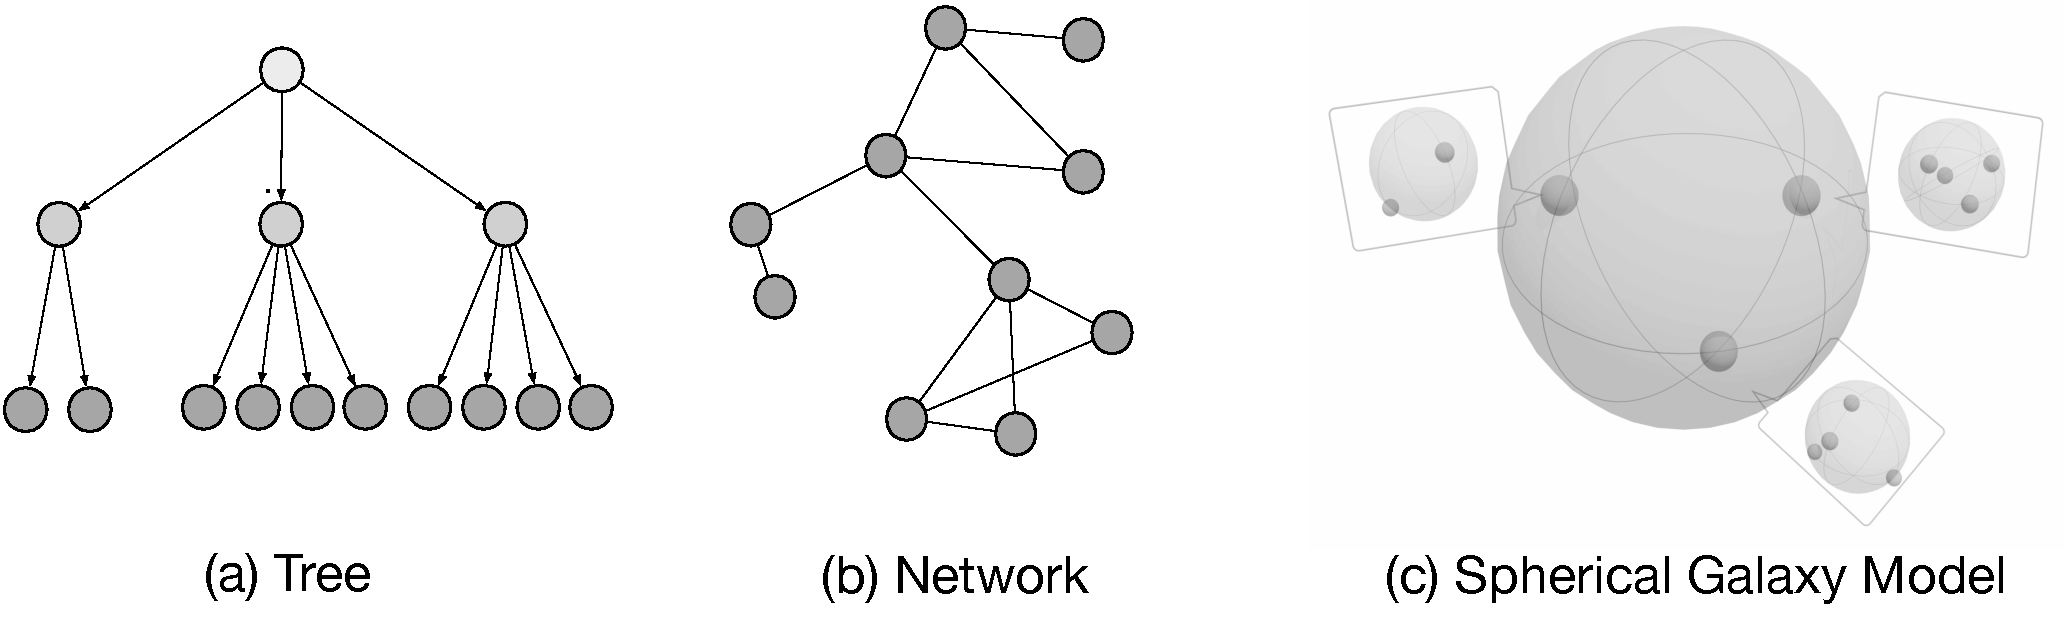
\includegraphics[width=0.95\linewidth]{figure/Galaxy.pdf}
			\caption{Different display approaches of the network hierarchical structure.}
			\label{fig:intuition}
		\end{figure}

\section{Related Work}
	\textbf{Network Embedding.} Network embedding maps the vertices or edges of a network into a low-dimensional vector space, which is beneficial at vertex classification and network visualization. 
	%Lots of excellent works are developed on learning the network representation. 
	It is well recognized that network representation has the two goals: reconstruction original network and support network inference. Manifold learning aims to reconstruct all the links, causing overfitting and limiting the network inference ability seriously\cite{Tenenbaum2000A}\cite{Roweis2000Nonlinear}.
	%for example, Isomap\cite{Tenenbaum2000A} preserves the geodesic distance of the data pairs. LLE\cite{Roweis2000Nonlinear} preserve the relationship of adjacent pairs. 
	In order to support network inference, structure-preserving method and property-preserving method are proposed. Our paper focuses on preserving structure information. Thus, in terms of structure-preserving methods, inspired by the word2vec in NLP\cite{mikolov2013efficient}, some methods consider the node context and represent a node with its nearby nodes. 
	For example, Deepwalk \cite{Perozzi2014DeepWalk} 
	%reveals that the distribution of vertices appearing in short random walk follows a power-law, similar with the distribution of words in natural languages. Thus, it 
	combines truncated random walk \cite{fouss2007random-walk} with the Skip-Gram \cite{mikolov2013efficient} to learn vertex representations; 
	Based on DeepWalk, Node2Vec \cite{Grover2016node2vec} proposes a biased random walk.
	%Node2Vec \cite{Grover2016node2vec} designs a kind of flexible network neighbourhood sampling strategy and proposes a biased random walk to learn vertex representations with Skip-Gram. 
	Another methods present more explicit optimization to preserve the pair-wise proximity of node, which take full account of the characteristics of network structures. For instance, LINE \cite{Tang2015LINE} formulates a novel optimization problem based on first- and second-order proximity on network embedding. GraRep \cite{Cao2015GraRep} integrate the $k$-step information to learn vertex representations.
	In addition to preserving the microscopic structure, the community structure, one important mesoscopic description of network structure, is incorporated into network embedding in MNMF\cite{Wang2017Community}.
	All the methods above mainly focus on preserving the pairwise proximity or community structure on a particular resolution, however, the community structure on different resolutions are not considered.

	 

	\textbf{Hierarchical Network.} Actually, many complex networks in the real world have hierarchical community structure. 
	\cite{newman2003structure} introduces the community structure of the network, and summarizes that complex networks have the small-world property and the scale-free property. \cite{song2005self} finds that a large number of real networks have the self-similar property. 
	Since the concept of community structure becomes richer in the presence of hierarchy, more and more works pay attention to extract hierarchy of networks.
	\cite{clauset2008hierarchical}
	\cite{Yang2013Hierarchical}\cite{sales-pardo2007extracting}\cite{Lancichinetti2008Detecting} propose effective approaches to extract hierarchical community structrue from complex networks that we can directly use in our model.
	Embedding the hierarchical community structure into low-dimensional vector spaces has not been investigated yet.

	\section{Problem Definition}
		We first give the definition of the hierarchical clustering tree \cite{clauset2008hierarchical} of a network.
		\begin{defn}[\textbf{\emph{Hierarchical Clustering Tree of Network}}]
			Given an undirected network $G = (V, E)$, the hierarchical clustering tree of $G$ is denoted as $T$ with a depth of $L$. $C$ is denoted as the node set,
			% as well as the community set of $G$. 
			$C^l$ as the node set at the $l$-th level and $c^l_i$ as the $i$-th node at the $l$-th level of $T$. $\Gamma(c)$ denotes the child node set of the node $c$ and $\delta(c)$ denotes the parent node of $c$. Meanwhile, $c^l_i$ also represents the $i$-th community while recursively dividing $G$ at the $l$-th level. For the $l$-th level of $T$,
				\[
				\forall c^l_i, c^l_j \in C^l \quad c^l_i \cap c^l_j = \varnothing
				\]
				\[
				\bigcup_i c_i^l = V.
				\]
			Especially, $c_1^1$ is the root node of $T$ and also the node set of $G$ (i.e. $c_1^1 = V$) and $c_i^L = \{v_i\}$, where $v_i$ is the $i$-th vertex of the $G$.
		\end{defn}
			%For brevity, we use $T$ to denote $T_G$. The notations of the variables used in the following paragraph are given here:  
		
		In order to preserve the hierarchical structure property of the network explicitly, we embed not only the vertices but also the communities of all levels. Due to $c_i^L = \{v_i\}$, 
		%\origin{Therefore, our model can preserve the structure property on all resolutions. As a community of $G$, the leaf node $c_i^L$ contains only one vertex $v_i$, thus the representation of $v_i$ is equivalent to $c_i^L$. }
		for brevity, we use community representation instead of vertex representation in the model. We define the community representation:
		\begin{defn}[\textbf{\emph{Community Representation}}]
			Given a network $G$ and its hierarchical clustering tree $T_G$, the community representation is a function $\mathcal{F}: C \rightarrow R^m$ ($m \ll |C|$) which can preserve the structure property of $G$.
		\end{defn} 
	    In our scenario, the community representation can preserve two kinds of properties of $G$. One is the local information, i.e. the pairwise proximity between sub-communities in the same community.
	    %\origin{(i.e. the pairwise proximity between the child nodes deriving from the same parent node in $T$)}. 
	    The other is the hierarchical structure property, i.e. the parent-child relationship and siblings relationship.
	    %contained in the tree structure. The formalized definition of the two properties will be given in the following paragraph. 
	    In order to preserve the local information between communities, we introduce the community proximity extended from the definition of the common neighbour similarity \cite{libennowell2007the}:
	    \begin{defn}[\textbf{\emph{Community Proximity}}]
			Community proximity is the pairwise similarity between communities in a network. 
			%It can be calculated according to the average similarity of the members belonging to different communities. Based on common neighbour similarity, 
			We define the proximity between $c^l_i$ and $c^l_j$.
			\begin{equation}
			S_{i,j}^k = \frac{1}{|c_i^l||c_j^l|}\sum_{u \in c_i^l} \sum_{v \in c_j^l} \xi_{u, v}
			\end{equation} 
			where $c_i^l, c_j^l \in \Gamma(c_k^{l-1})$
			and $\xi_{u, v}$ is the similarity between the vertex pair $u$ and $v$ shown as follows :
			\begin{equation}
			\xi_{u,v} = \frac{A_u^TA_v}{\sqrt{||A_u||_1||A_v||_1}},
			\end{equation}
			where $A$ is the adjacency matrix of $G$, $A_u$ is the $u$-th column of the $A$.	
		\end{defn}
		%\begin{defn}[\textbf{\emph{Community Proximity}}]
		%	Community proximity is the pairwise similarity between communities in a network. It can be calculated according to the average similarity of the members belonging to different communities. Based on common neighbour similarity, We define the proximity between $c^l_i$ and $c^l_j$.
		%	\begin{equation}
		%	S_{i,j}^k = \frac{1}{|c_i^l||c_j^l|}\sum_{u \in c_i^l} \sum_{v \in c_j^l} \xi_{u, v}
		%	\end{equation} 
		%	where $c_i^l, c_j^l \in \Gamma(c_k^{l-1})$
		%	and $\xi_{u, v}$ is the similarity between the vertex pair $u$ and $v$ shown as follows :
		%	\begin{equation}
		%	\xi_{u,v} = \frac{A_u^TA_v}{\sqrt{||A_u||_1||A_v||_1}},
		%	\end{equation}
		%	where $A$ is the adjacency matrix of $G$, $A_u$ is the $u$-th column of the $A$.	
		%\end{defn}
		%Taking community proximity preservation into consideration, 
 
	\section{Galaxy Network Embedding Model}
	\label{sec:model}
	%Inspired by the structure of galaxies, the original optimization(see Eq.\ref{equ:whole_loss}) is transformed into an optimization with spherical constraints(see Eq.\ref{equ:local_objective}). In particular, we design a determination strategy of radii and propose a spherical embedding method for sphere of each layer in hierarchy. Finally, the algorithm of the GNE can be found in the last part of this section.  
	 %\subsubsection{Properties of Galaxy Structure}
	 
	 The galaxy, another type of systems with hierarchical structure, has two desirable structural characteristics which ensure that the embedding results preserve the essence of hierarchy(see Fig.\ref{fig:structure}): The first is that stars belonging to the same galaxy distribute in the sphere of ball almostly; The other is that the distance between two galaxies is much larger than the radius of each of them.
	 
	 \subsection{Hierarchical Preserving Network Embedding}
	 Firstly, we introduce pairwise optimization objective which extends 1-step optimization objective in GraRep \cite{Cao2015GraRep}. To preserve the proximity between communities deriving from the same parent node $c_k^{l-1}$, the KL-divergence should be minimized between the distribution of community similarity from ground truth and learned representation respectively: 
			\begin{equation}
			\label{equ:local_loss} 
			\begin{split}
			O^{(k)}(\Phi, \Phi') & = \sum_{c_i^l, c_j^l \in \Gamma(c_k^{l-1})} \frac{S_{i,j}^l}{\sum_t S_{i, t}^l} \cdot \log{\sigma(\Phi(c_i^l)^T \Phi'(c_j^l))} \\
			+ \frac{\lambda}{|\Gamma(c_k^{l-1})|}&\sum_{c_e^l \in \Gamma(c_k^{l-1})} \frac{S_{i, e}^l}{\sum_t S_{i, t}^l} \cdot \log{\sigma(-\Phi(c_i^l)^T \Phi'(c_e^l))}, \\
			\end{split}
			\end{equation}
	where $\sigma(\cdot)$ is the sigmoid function, $\Phi(c)$ is the `current' vector of community $c$ we want and $\Phi'(c)$ is the `context' vector of community $c$ which is an auxiliary variable. $\lambda$ is a hyper-parameter related to negtive sampling indicating the number of negative samples.

	Inspired by the galaxy structure, the hierarchical preserving network embedding problem is formally defined as a constrained optimization problem:
			\begin{equation}
			\label{equ:whole_loss}
			\begin{split}
			\min_{\Phi,\Phi'} & \sum_l^{L-1}\sum_{c^k_l \in C^l} O^{(k)}(\Phi, \Phi') \\
			s.t. \quad
			|| \Phi(c_u^l) - & \Phi(c_v^l) || - ||\Phi(c_u^l) - \Phi(c_w^l)|| < 0, \\
			|| \Phi(c_i^{l+1}) - & \Phi(c_j^{l})) || - ||\Phi(c_j^{l}) - \Phi(c_k^{l - 1})|| < 0,\\
			\end{split}
			\end{equation}
			where,
			\[
			\begin{split}
				\delta(c_u^l) = \delta(c_v^l), \quad \delta(c_u^l) \neq \delta(c_w^l)\\
				\delta(c_i^{l+1}) = c^l_j, \quad \delta(c^l_j) = c^{l - 1}_k \\ 
			\end{split}
			\]
		The constraints can be divided into two aspects: Horizontally, vertices belonging to the same community should be closer to each other than those belonging to different communities (see the first constraint). 
		Vertically, the cohesion degree of low level communities should be less than that of high level ones in $T$ (see the second constraint). 
	
		It can be seen that the constrained optimization objective Eq.\ref{equ:whole_loss} is very complex, the number of whose constraints reaches $O (|V|^3) $. It is hard to solve the optimization problem directly.

	 %\subsection{Model Framework based on Galaxy Structure}
	 \subsection{Galaxy Network Embedding}
	 We introduce stronger constraints and suppose galaxies are located at a spherical surface to simplify the objective Eq.\ref{equ:whole_loss}. In other words, the distances from each galaxy to the center of its galaxy group are equal. Besides the Euclidean representation $\Phi(c_i^l)$, each embedded community $c_i^l$ has another attribute $r_i^l$ (the radius of the corresponding galaxy group).
	 We have the following constraints:

	 \begin{equation}
	 \begin{split}
	 	\label{equ:sphere_constraints}
	 	\forall c_v^{l+1} & \in \Gamma(c_i^l), \quad l = 1, 2, ..., L - 1,\\
	 	& ||\Phi(c_v^{l+1})  - \Phi(c_i^l)||_2= r_i^l, \\	
	 \end{split}
	 \end{equation}
	 \begin{equation}
	 \label{equ:galaxy_constraints}
	 	\sum_{j=l}^L r^j < \zeta d^{l-1}_{i, *}, \quad \zeta < \frac{1}{5}	 	
	 \end{equation}
	 where,
	 \[
	 d_{i, *}^{l-1} = \min_{c_j^l \in \Gamma(\delta(c_i^l)), i \neq j} ||\Phi(c_i^l)-\Phi(c_j^l)||
	 \]

	 Especially, $L$ denotes the depth of $T_G$ and $\zeta$ is a constant that guarantees any two spherical surfaces at any layer are not intersected.

	 \begin{lem}
	 The cooccurrence of Eq.\ref{equ:sphere_constraints} and Eq.\ref{equ:galaxy_constraints} is a sufficient case of the presence of constraints in the objective Eq.\ref{equ:whole_loss}.
	 \end{lem}
	 \begin{proof}
	 if Eq.\ref{equ:sphere_constraints} and Eq.\ref{equ:galaxy_constraints} are satisfied simultaneously:

	 $\Rightarrow$ The first constraint in Eq.\ref{equ:whole_loss} can be satisfied, i.e.:
	 \[
	 	\lVert \Phi(c_u^{l}) - \Phi(c_v^{l})\rVert_2 - \lVert\Phi(c_u^{l}) - \Phi(c_w^{l})\rVert_2 < 0
	 \]
	 where
	 \[
	 	c_u^{l+1}, c_v^{l+1} \in \Gamma{(c_i^l)}, \quad c_w^{l+1} \in \Gamma{(c_j^l)}
	 \]
	 Obviously, 
	 \[
	 \begin{split}
	 	\lVert \Phi(c_u^{l}) - \Phi(c_v^{l})\rVert_2 &< 2\max{(r_i^l, r_j^l)} \\
	 	\lVert\Phi(c_u^{l}) - \Phi(c_w^{l})\rVert_2 &> d_{i, j}^{l-1} - 2\max{(r_i^l, r_j^l)} 
	 \end{split}
	 \]
	 According to the Eq.\ref{equ:galaxy_constraints},
	 \[
	 	\lVert \Phi(c_u^{l}) - \Phi(c_v^{l})\rVert_2 - \lVert\Phi(c_u^{l}) - \Phi(c_w^{l})\rVert_2 < 0
	 \]
	 Thus, the first constraint in Eq.\ref{equ:whole_loss} can be satisfied.

	 $\Rightarrow$ The second constraint in Eq.\ref{equ:whole_loss} can be satisfied, i.e.
	 \[
	 	\lVert\Phi(c_v^{l+1}) - \Phi(c_i^{l})\rVert_2 - \lVert\Phi(c_i^{l}) - \Phi(c_k^{l-1})\rVert_2 < 0
	 \]
	 where,
	 \[
	 	\lVert\Phi(c_v^{l+1}) - \Phi(c_i^{l})\rVert_2 = r_i^l, \quad \lVert\Phi(c_i^l) - \Phi(c_k^{l-1})\rVert_2 = r_k^{l-1}
	 \]
	 and according to Eq.\ref{equ:galaxy_constraints}, we have:
	 \[
	 	\begin{split}
	 	r_i^l < \zeta d_{i, *}^{l-1} &\leq 2\zeta r_k^{l-1}, \quad \zeta < \frac{1}{5} \\
	 	\Rightarrow \lVert\Phi(c_v^{l+1}) - \Phi(&c_i^{l})\rVert_2 < \lVert\Phi(c_i^{l}) - \Phi(c_k^{l})\rVert_2\\
	 	\end{split}
	 \]
	 In conclusion, the constraints of Eq.\ref{equ:whole_loss} can be satisfied if Eq.\ref{equ:sphere_constraints} and Eq.\ref{equ:galaxy_constraints} are satisfied.
	 \end{proof}

	
	\subsubsection{Objective of Galaxy Network Embedding Model}
	Next, we define the GNE optimization objective with $c_k^{l-1}$ as the parent community:
	\begin{equation}
	  \label{equ:local_objective}
	  \begin{split}
	  O^{(k)}(\Phi, \Phi') & = \sum_{c_i^l, c_j^l \in \Gamma(c_k^{l-1})} \frac{S_{i,j}^l}{\sum_t S_{i, t}^l} \cdot \log{\sigma(\Phi(c_i^l)^T \Phi'(c_j^l))} \\
		 + \frac{\lambda}{\lvert\Gamma(c_k^{l-1})\rvert}&\sum_{c_e^l \in \Gamma(c_k^{l-1})} \frac{S_{i, e}^l}{\sum_t S_{i, t}^l} \cdot \log{\sigma(-\Phi(c_i^l)^T \Phi'(c_e^l))}, \\
		 \\
		s.t. \quad \forall c_i^{l+1} & \in \Gamma(c_k^l),\quad \lVert \Phi(c_i^{l+1})  - \Phi(c_k^l)\rVert_2= r_k^l \\
	  \end{split}
	  \end{equation}
	%Besides, we design a proper determination strategy of $r_i^l$ for each community $c_i^l$.
	where, the radius $r_k^l$ for each community $c_k^l$ can be obtained with a proper determination strategy introduced next. In this way, we can optimize the objective Eq.\ref{equ:local_objective} recursively from top to bottom in hierarchy. The whole embedding procedure is illustrated in Fig.\ref{fig:structure}. 

	\begin{figure}[ht]
	 	\centering
		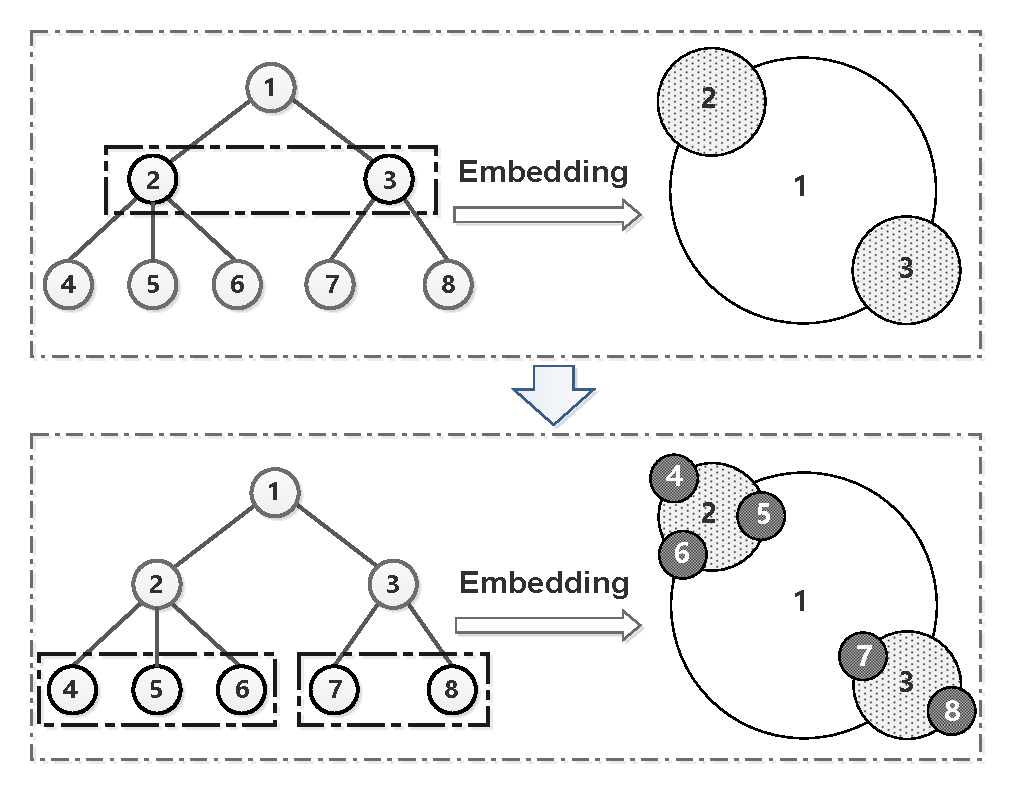
\includegraphics[width=0.6\linewidth]{figure/Structure.pdf}
		\caption{Structure of GNE}
		\label{fig:structure}
	 \end{figure}

	 \section{Learning Procedure of GNE}
	 In this section, we introduce the learning algorithm of GNE, including how to solve the optimization problem Eq.\ref{equ:local_objective} layer by layer and how to obtain the radius of each community.

	 \subsection{Spherical Embedding Algorithm}
	 Compared with the optimization objective of the classic neural embedding method, we just add an extra spherical constraint in Eq.\ref{equ:local_objective}. The neural embedding method can be directly optimized using SGD, which is efficient and whose effect has been verified. Considering these advantages, we transform Eq.\ref{equ:local_objective} into a two-step optimization procedure. First, we use the Adam optimizer \cite{Rushing2005ADaM} to optimize Eq.\ref{equ:local_loss} without constraint based on neural networks, and obtain the intermediate representation $\Omega(c^l_i)$ of communities which preserving the pairwise relative Euclidean distances of communities. Second, we map $\Omega(c^l_i)$ to a spherical surface to get the final representation $\Phi(c_i^l)$ of communities. Next, we introduce the spherical projection method.

	 \subsubsection{Optimization Objective of Spherical Projection}
	 To preserve the relative distances in spherical projection, we formally define the following optimization objective: 

    \begin{equation}
    \label{equ:sphere_objective}
    \begin{split}
    \min_{\Phi} J^{(k)} =  & \left\lVert\frac{D}{\lVert D \rVert_F} - \frac{B}{\lVert B \rVert_F}\right\rVert_F + \mu \exp(- \gamma \lVert B \rVert_F)\\ 
    & s.t. \lVert \Phi(c_i^{l})  - \Phi(c_k^{l-1})\rVert= r_k^{l-1}\\
    \end{split}
    \end{equation}
	 where,
	 \[
	 \begin{split}
	 	c_i^l,c_j^l &\in \Gamma(c_k^{l-1})\\
	 	D_{ij} = \lVert \Omega(c^{l}_i) - \Omega(c^{l}_j)\rVert &\quad B_{ij} = \lVert \Phi(c^{l}_i) - \Phi(c^{l}_j)\rVert \\
	 \end{split}
	 \]
	 The first term is to preserve the relative distances, and the second term is a penalty term to make the distances between each pair of points after projection are as large as possible. $\mu$ and $\gamma$ are hyper parameters. As the overall optimization procedure is top-down, $\Phi(c_k^{l-1})$, $r_k^{l-1}$ and $D$ are all constants. 
   
    \subsubsection{Spherical Projection Optimization Procedure}
    The constraints of Eq.\ref{equ:sphere_objective} are for arbitrary spherical surfaces. We can perform scaling and translation transformations on the coordinate system to turn them into the unit sphere constraints, namely the following conversion :
    \begin{equation}
    	\label{equ:transfer}
    	\Psi(c_i^l) = \frac{\Phi(c_i^l) - \Phi(c_k^{l-1})}{r_k^{l-1}}, \quad and \quad \lVert \Psi(c_i^l) \rVert = 1.
    \end{equation}
    %Hence the constraints can be transformed as follows:
   % \begin{equation}
    %\label{equ:unit}
    %	\lVert \Psi(c_i^l) \rVert = 1.
    %\end{equation}
    Combining with Eq.\ref{equ:transfer}, the Euclidean distance between $\Psi(c_i^{l})$ and $\Psi(c_j^l)$ can be expanded as follows: 
    \begin{equation}
    \begin{split}
    \label{equ:bij}
    	B_{ij}' &= \lVert \Psi(c_i^{l}) - \Psi(c_j^l) \rVert \\
    			&= \lVert \Psi(c_i^l) \rVert^2 + \lVert \Psi(c_j^l) \rVert^2 - 2 \Psi(c_i^l)^T \Psi(c_j^l) \\
    			&= 2 - 2\cos(\Psi(c_i^l), \Psi(c_j^l)) \\
    \end{split}
    \end{equation}
    %Bringing Eq.\ref{equ:unit} into Eq.\ref{equ:bij}, we have:
    %\begin{equation}
    %\begin{split}
    %	B_{ij}' = & \lVert \Psi(c_i^l) \rVert^2 + \lVert \Psi(c_j^l) \rVert^2 - 2 \Psi(c_i^l)^T \Psi(c_j^l) \\
    %	= & 2 - 2\cos(\Psi(c_i^l), \Psi(c_j^l))
    %\end{split}
    %\end{equation}
    It can be seen that $B_{ij}'$ is not related to the length of vector $\Psi(c_i^l)$ and $\Psi(c_j^l)$, but only the Cosine distance between them. Therefore, the vector length constraint in the objective can be removed. The final optimization objective on the unit sphere is: 
    \begin{equation}
	 	\label{equ:unit_sphere_objective}
            \min_{\Psi} H^{(k)} = \left\lVert\frac{D}{\lVert D \rVert_F} - \frac{B'}{\lVert B' \rVert_F}\right\rVert_F + \mu \exp(- \gamma \lVert B' \rVert_F). 
    \end{equation}
    We use $\Psi_*(c_i^l)$ to denote the minimum point after optimization. After normalization, translation, and scaling, the final results are obtained: 
    \begin{equation}
    	\label{equ:sphere_transformation}
    	\Phi(c_i^l) = \frac{\Psi_*(c_i^l)}{\lVert \Psi_*(c_i^l) \rVert} \times r_k^{l-1} + \Phi(c_k^{l-1}) 
    \end{equation}
    Obviously, the unconstrained objective has a lower bound that can be found using Gradient Descent algorithm.

	 \subsection{Strategy of Determining Radius}
	 According to Eq.\ref{equ:galaxy_constraints}, the radius $r$ and the distance $d$ between two spheres should be subject to:
	 \begin{equation}
	 	\label{equ:r_and_eta}
	 	r_i^l= \eta \dot d_{i, *}^{l-1}, \quad \eta < \frac{1}{2}
	 \end{equation}
	 where
 	 \begin{align}
 		\label{equ:mind}
 		d_{i,*}^{l-1} = \min_{c^{l}_j \in \Gamma(\delta(c^{l}_i)), i \neq j}& \lVert\Phi(c_i^{l}) - \Phi(c_j^{l})\rVert \\
 		\label{equ:d_and_r}
 		d_{i,*}^{l-1} <& 2 \cdot r_i^{l-1}
 	\end{align}
 	More precisely, $r^l$ denotes the sphere radius of nodes at layer $l$ and $\eta$ reflects the cohesion degree of the community $c_i^l$ relative to $c_*^l$.

	 \begin{lem}
	 \label{prf:eta}
	 	When $\eta$ is less than $\frac{\zeta}{1+2\zeta}$, the constraint Eq.\ref{equ:galaxy_constraints} can be satisfied, where $\zeta$ is a constant to make sure any two spherical surfaces at any layer will not intersect in Eq.\ref{equ:galaxy_constraints}. 
	 \end{lem}
	 \begin{proof} 
	 	According to Eq.\ref{equ:r_and_eta} and Eq.\ref{equ:d_and_r}, the relationship between $r^j$ and $d_*^{l-1}$ can be derived as follows, where $j \in [l, L]$:	
	 	\begin{align}
	 	\label{equ:derivation}
	 		\nonumber
	 		r^j &= \eta \cdot d_*^{j-1} < \eta \cdot 2r^{j-1} \\
	 		\nonumber
	 		&= 2\eta^2 \cdot d_*^{j-2} < 2^2\eta^2 \cdot r^{j-2} \\
	 		\nonumber
	 		&... ...\\
	 		&< 2^{k-1}\eta^k \cdot d_*^{j-k}
	 	\end{align}
	 	When $k=j-l+1$, 
	 	\begin{equation}
	 		\label{equ:j_and_l}
	 		r^j < 2^{j-l}\eta^{j-l+1} \cdot d_*^{l-1}
	 	\end{equation}
	 	thus, we get the upper bound of $r^j$. The inequation Eq.\ref{equ:galaxy_constraints} is valid if the upper bound of $\sum r^j$ is less than $\zeta d_*^{l-1}$. Substituting Eq.\ref{equ:galaxy_constraints} for Eq.\ref{equ:j_and_l}, we obtain:
	 	\begin{equation}
	 	\nonumber
	 	\sum_{j=l}^L 2^{j-l} \eta^{j-l+1} \cdot d_*^{l-1} < \zeta d_*^{l-1} \Rightarrow \sum_{j=l}^L r^j < \zeta d_*^{l-1} 
	 	\end{equation}
	 	Thus, since $\eta < \frac{1}{2}$ , 
	 	\begin{align}
	 	\nonumber
	 	\sum_{j=l}^L (2\eta)^{j-l+1}& < \frac{2\eta}{1-2\eta}< 2 \zeta \\
	 	\nonumber
	 	\Rightarrow \eta <& \frac{\zeta}{1+2\zeta}
	 	\end{align}
	 	In conclusion, when $\eta < \frac{\zeta}{1+2\zeta}$, the objective of GNE model (Eq.\ref{equ:galaxy_constraints}) is equivalent to the original objective (see Eq.\ref{equ:whole_loss}).
	 \end{proof}

    \subsection{The GNE Algorithm}
	The pseudocode for GNE, is given in Algorithm \ref{alg:gne}. The whole embedding process is executed from top to down. For all children nodes of a certain node $c_i^l$, i.e. the nodes in $\Gamma(c_i^{l})$, the learned representation $\Psi(\Gamma(c_i^{l}))$ on the unit sphere can be obtain after two-step optimization procedure with Adam\cite{Rushing2005ADaM}, the optimization Eq.\ref{equ:local_loss} is used first and the optimization Eq.\ref{equ:unit_sphere_objective} follows.
    The final representation $\Phi(c_j^{l+1})$ can be obtained by the transformation in Eq.\ref{equ:sphere_transformation}. Besides, the corresponding $r_j^{l+1}$ can be calculated with minimum distance $d_{j,*}$ and a constant $\eta$ less than $\frac{1}{5}$ (see Lemma \ref{prf:eta}).
    
    \begin{algorithm}[H] 
\caption{The GNE algorithm} 
	\label{alg:gne} 
\begin{algorithmic}
\Function{LearnFeatures}{Network $G$, Hierarchical Clustering Tree $T$}
	\State Initialize $\Phi(c^1_1) = 0$ and $\bf{r_1^1} = 1$
	\State $\bf{\Phi}$ = OptimizeRecursively($c_1^1$, $G$, $T$, $\bf{r}$, $\bf{\Phi}$) \\
	\Return $\bf{\Phi}$ 
\EndFunction
	\\\hrulefill
\Function{OptimizeRecursively}{Current node $c^l_i$, Network $G$, Hierachical Clustering Tree $T$, Radius Set $\bf{r}$, Reresentation Set $\bf{\Phi}$} 
	\If{$l = L$}
		\Return $\bf{\Phi}$		
	\EndIf
	\State $\Omega(\Gamma(c_i^{l}))$ = Optimize Objective $O^{(i)}$ with Adam
	\State $\Psi(\Gamma(c_i^{l}))$ = Optimize Objective $H^{(i)}$ with Adam
	\ForAll{$c_j^{l+1} \in \Gamma(c_i^l)$}
		\State $\Phi(c_j^{l+1}) = \frac{\Psi(c_j^{l+1})}{\lVert \Psi(c_j^{l+1}) \rVert}  \times \bf{r_i^{l}} + \Phi(c_i^{1})$
		\State $\bf{r_j^{l+1}} = \eta \cdot d_{j,*}$
	\EndFor
	\ForAll{$c_j^{l+1} \in \Gamma(c_i^l)$}
		\State $\bf{\Phi}$ = OptimizeRecursively($c_j^{l+1}$, $G$, $T$, $\bf{r}$, $\bf{\Phi}$) 
	\EndFor
	\Return $\bf{\Phi}$
\EndFunction
\end{algorithmic} 
\end{algorithm}

    \subsubsection{Time Complexity Analysis}
    For brevity on description, we assume that the hierarchical clustering tree of network $G=(V,E)$ is a k-ary tree $T_G$ with depth $log_K|V|$. The number of nodes N in $T_G$ is $\frac{K^{log_K|V|+1} -1}{K-1}$. Spherical embedding should be done on each tree node layer by layer. Especially, the embedding procedures on the same layer tree nodes can be parallelized. For spherical embedding, the complexity of computing $\Omega(\Gamma(c_i^{l}))$ is $O(\mathcal{E} \times K \times Q)$. More precisely, $\mathcal{E}$ is the number of training epoch, $K$ is the size of community to be embedded and $Q$ is the neural network computing complexity of skip-gram model, i.e. $Q=O(C \times (\mathcal{D}+\mathcal{D} \times M))$, where $C$ is the skip window size, $\mathcal{D}$ is the embedding size and $M$ is the negative sampling size; the complexity of computing $\Psi(\Gamma(c_i^{l}))$ is $O(\mathcal{E} \times K^2 \times \mathcal{D})$. Thus, the spherical embedding complexity is $O(\mathcal{E} \times K \times Q + \mathcal{E} \times K^2 \times \mathcal{D})$. The optimization algorithm is implemented on the Tensorflow platform, which can be accelerated with GPU.

\section{Experiments}
	In this section, An experimental analysis of our method on both synthetic and real networks is presented. The code of our model is available on Github.
	
	\begin{table*}[!h]
	\centering
	\resizebox{\textwidth}{!}{%
	\begin{tabular}{|c|c|c|c|c|c||c|c|c|c|c||c|c|c|c|c|}
	\hline
	Model &
	\multicolumn{5}{c||}{Amherst} &
	\multicolumn{5}{c||}{Hamilton} &
	\multicolumn{5}{c|}{Georgetown} \\
	\hline
	&
	10\% & 30\% & 50\% & 70\% & 90\% &
	10\% & 30\% & 50\% & 70\% & 90\% &
	10\% & 30\% & 50\% & 70\% & 90\%
	\\
	\hline
	GNE & 
	\textbf{94.91} & \textbf{94.25}  &  \textbf{93.94} & \textbf{93.97} & \textbf{93.39} &
	\textbf{94.66} & \textbf{94.55}  &  \textbf{94.49}  &   \textbf{94.49}  &  \textbf{93.88} &
	53.57 & \textbf{53.79}  & 53.06 & \textbf{52.75} & \textbf{52.11}
	\\
	SpectralClustering &
	72.89 & 73.49 & 73.94 & 74.32 & 72.82 &
	78.16 & 77.60 & 77.21 & 77.59 & 74.92 &
	49.26 & 50.87 & 50.79 & 50.60 & 48.53
	\\
	DeepWalk &
	90.62 & 91.65 & 91.32 & 91.13 & 90.41 &
	92.89 & 92.33 & 92.52 & 92.18 & 91.55 &
	54.07 & \textbf{53.79} & 53.35 & 51.69 & 50.92
	\\ 
	Node2Vec &
	91.29 & 91.24 & 91.04 & 90.44 & 90.02 &
	92.09 & 91.03 & 91.18 & 90.06 & 89.56 &
	52.86 & 53.73 & 53.16 & 52.70 & 51.28 
	\\
	LINE &
	90.76 & 91.82 & 91.48 & 91.09 & 89.42 &
	92.33 & 92.72 & 92.52 & 92.62 & 91.73 &
	54.64 & 53.45 & 53.81 & 52.71 & 51.28
	\\
	GraRep &
	92.13 & 92.25 & 91.78 & 91.56 & 91.48 &
	93.67 & 93.04 & 92.30 & 92.40 & 91.00 &
	\textbf{54.80} & 53.24 & \textbf{53.95} & 51.87 & 51.74
	%\textbf{58.10} & \textbf{59.24} & \textbf{57.95} & \textbf{56.87} & \textbf{54.74}
	\\
	MNMF &
	89.82 &  89.06 & 88.04 & 86.43 & 78.44 &
	91.42 & 90.32 & 89.12 & 87.02 & 81.19 &
	53.43 & 52.63 & 52.10 & 51.52 & 50.35
	\\
	\hline
	\end{tabular}
	} %
	\caption{The multi-label classification results on different percentages of test data sets.}
	  \label{tab:classification}
	\end{table*}
 

	\subsection{Experiment Setup}

	\noindent \textbf{Data Sets} We employed the following three real datasets in Facebook social networks \cite{Traud2012Social} for node classification, which comprises 100 colleges and universities in US. We choose the social networks in Hamilton University(2314 nodes, 96394 edges), Amherst College(2235nodes, 90954edges) and Georgetown Universit(9414 nodes, 425639 edges). Besides, in order to evaluate the performance of hierarchical community structure preservation, four Hierarchical Random Graphs (HRG) with explicit hierarchical community structure are generated by \cite{clauset2008hierarchical}, i.e. Syn\_with\_125nodes(125 nodes, 406 edges), Syn\_with\_1800nodes(1800nodes, 739637 edges), Syn\_with\_2560nodes(2560 nodes, 1460147 edges) and Syn\_with\_3750nodes(3750 nodes, 3066250 edges).

	\noindent \textbf{Relevant Algorithms}
	We compared the GNE against the following six network embedding algorithm: SpectralClustering\cite{Tang2011Leveraging}, DeepWalk\cite{Perozzi2014DeepWalk}, Node2Vec\cite{Grover2016node2vec}, LINE\cite{Tang2015LINE}, GraRep\cite{Cao2015GraRep} and MNMF\cite{Wang2017Community}. Additionally, we extract the hierarchical community structure of networks with \cite{Tsvetovat2011Social} as the input of GNE.  

	\noindent \textbf{Parameters Settings} 
	The hyper-parameters of GNE is $\bm{\theta}$, i.e. $\bm{\theta}=(\lambda, \mu, \gamma)$. GNE is not very sensitive to the hyper-parameters, whose artificial settings can achieve ideal results with GridSearch as auxiliary on a small range. Besides, the parameter setting of comparison models follow the recommended settings in relevant code packages.

	\subsection{Hierarchical Community Detection}
	In this section, we verify the ability of hierarchical community preservation of our model GNE. We consider synthetic data sets in this experiment, including three different structure of HRG but with the same number of layers(see Fig.\ref{fig:community_preservation}). Besides, Jaccard's coefficient \cite{halkidi2001clustering} is applied as an external intex for evaluating the performance of community preservation at each hierarchy of networks.

	\begin{figure}[htbp]
		\center
		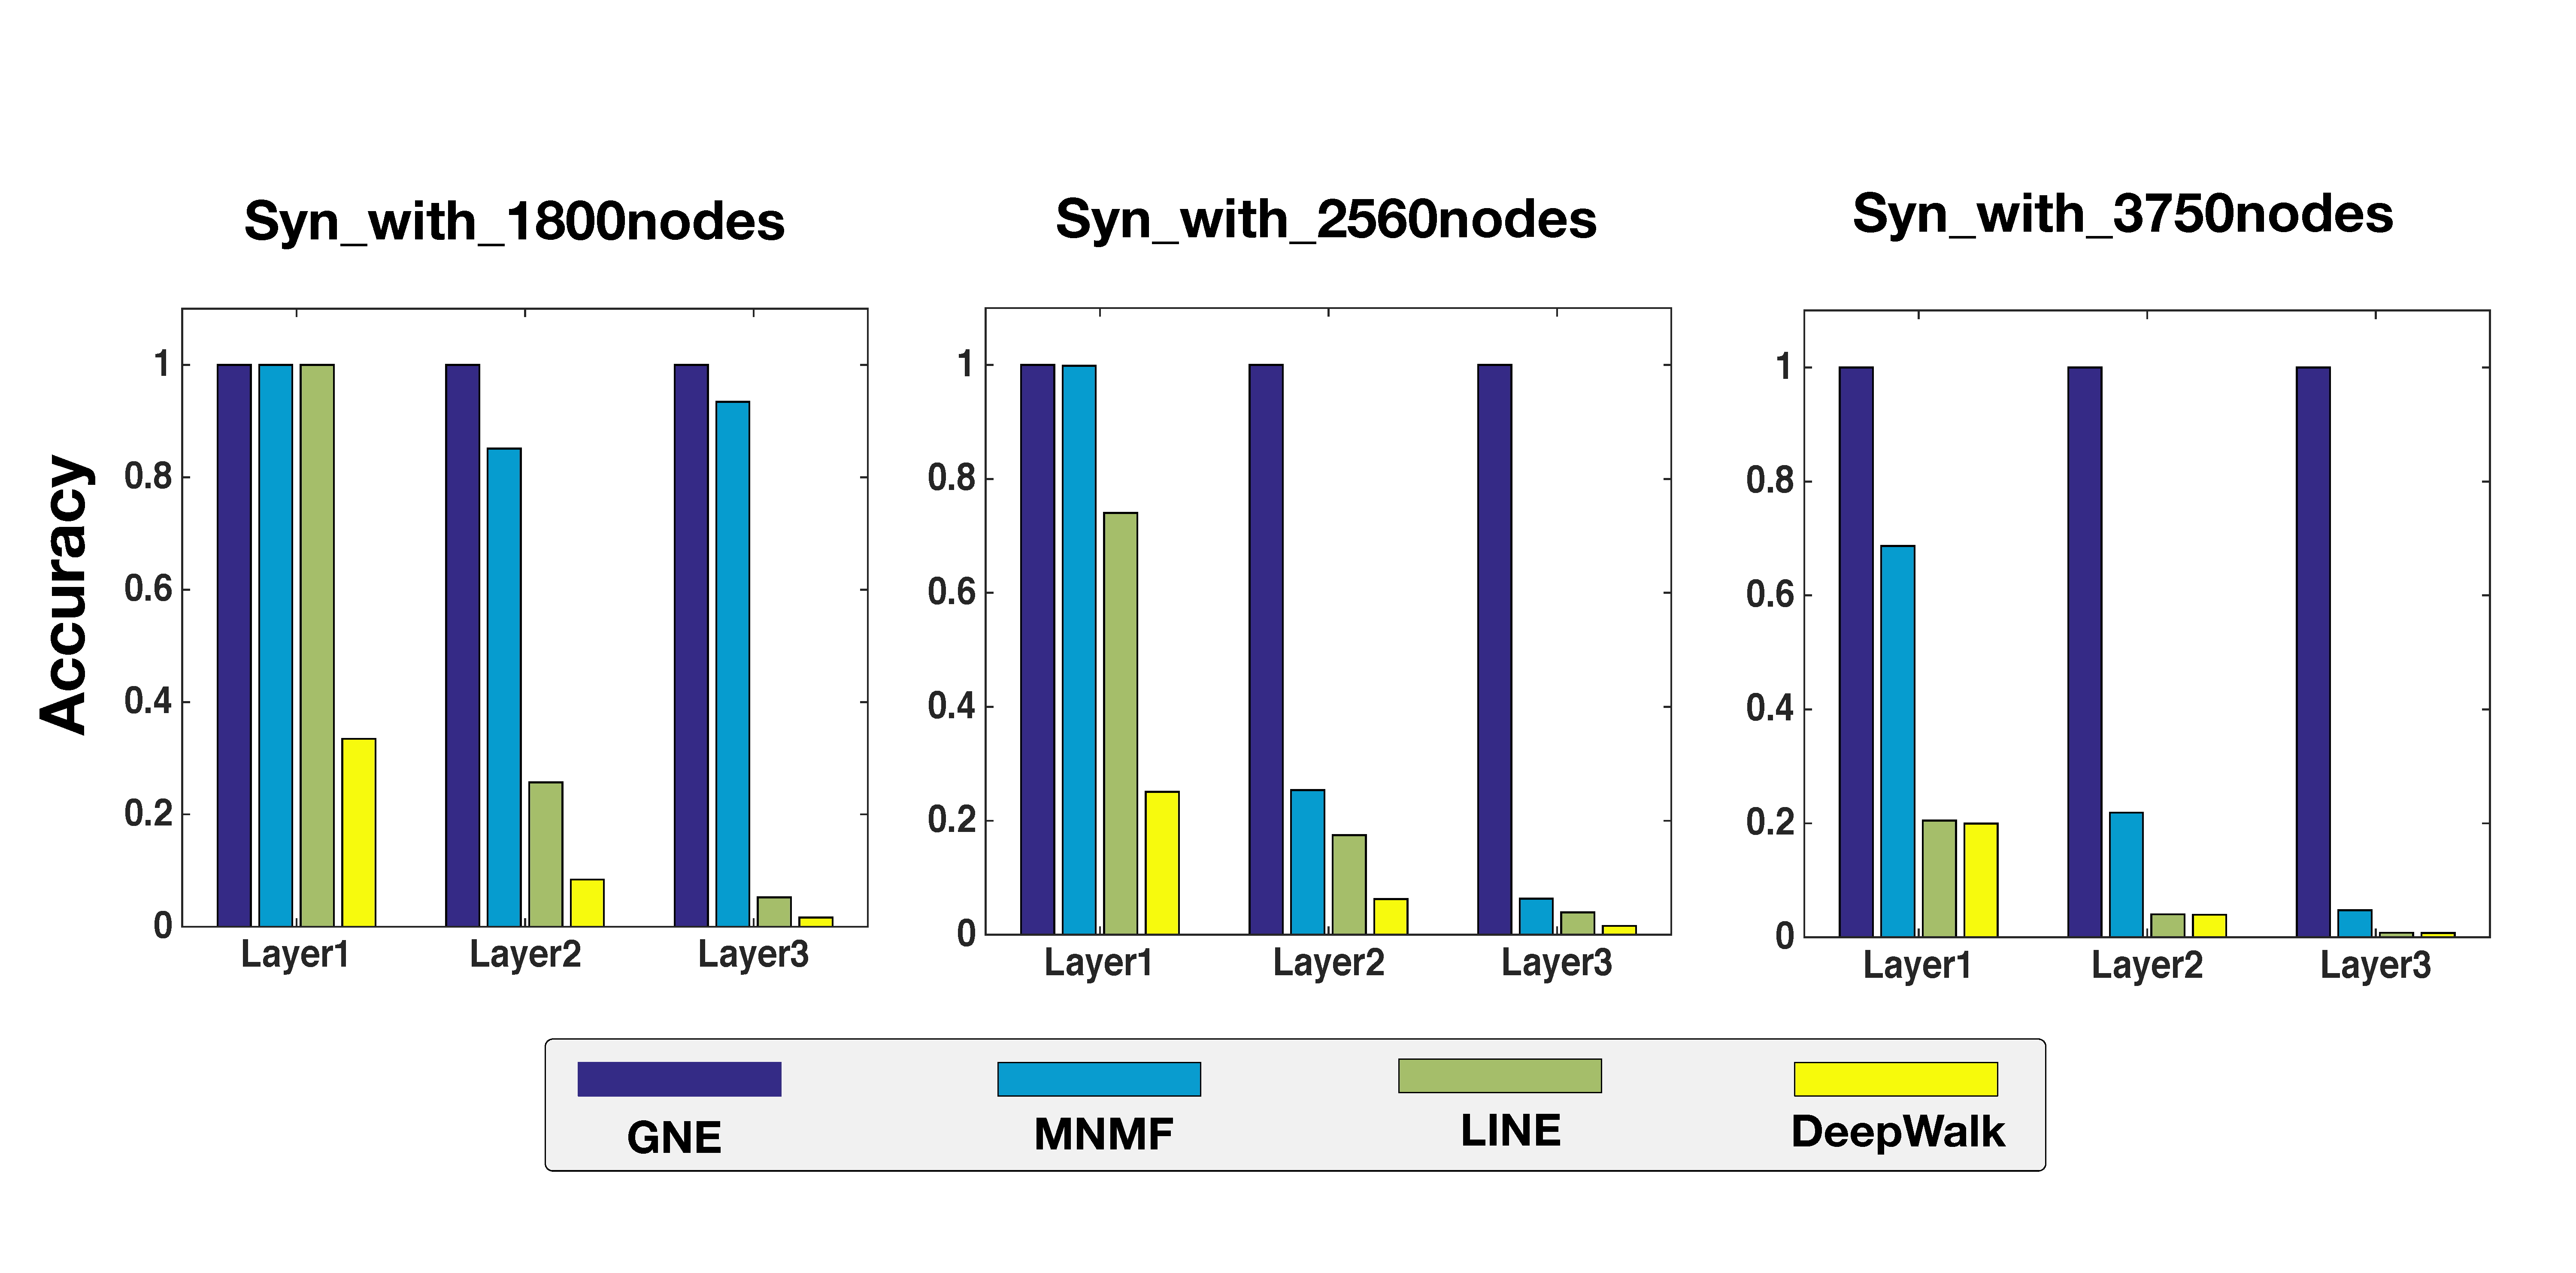
\includegraphics[width=0.5\textwidth]{figure/community_preservation.pdf}
		\caption{The comparision of hierarchical community preservation on different models. Three different structure of HRG but with the same number of layers are used. For each histogram, the horizontal ordinate denotes layer number, and the vertical ordinate denotes the Jaccard's coefficient.}
		\label{fig:community_preservation}
	\end{figure}
	Fig.\ref{fig:community_preservation} shows that the content of the hierarchical community structure can be integrally preserved with our model, no matter how many the number of communities is. However, MNMF preserving community information on a particular resolution is inferior to GNE, and the other model could not perfectly deal with such cases with multi-layer and complex community structure.

	\subsection{Network Visualization}
	Network visualization is an important application of network embedding which maps a network into two-dimensional space. We visualize a synthetic network with 125 nodes, 406 edges and 5 communities. Fig.\ref{fig:visualization} presents the visualization experiments. We firstly generate a self-similar network of which nodes are derived from the leaves of five-ary tree with four layers and edges are derived from the sampling of connected paths between leaves in the tree. Additionally, the nodes in the network are classified into different communities with Girvan–Newman algorithm \cite{girvan2002community}. We compare our method against other models.

	For other models, we layout the network into low-dimensional space, and then further map the low-dimensional vectors of the nodes to a 2-D space with t-SNE package \cite{Maaten2008Visualizing}. For our model, we can directly embed network into 2-D vector space according to hyper spherical embedding we proposed.

	\begin{figure}[htb]
		\center
		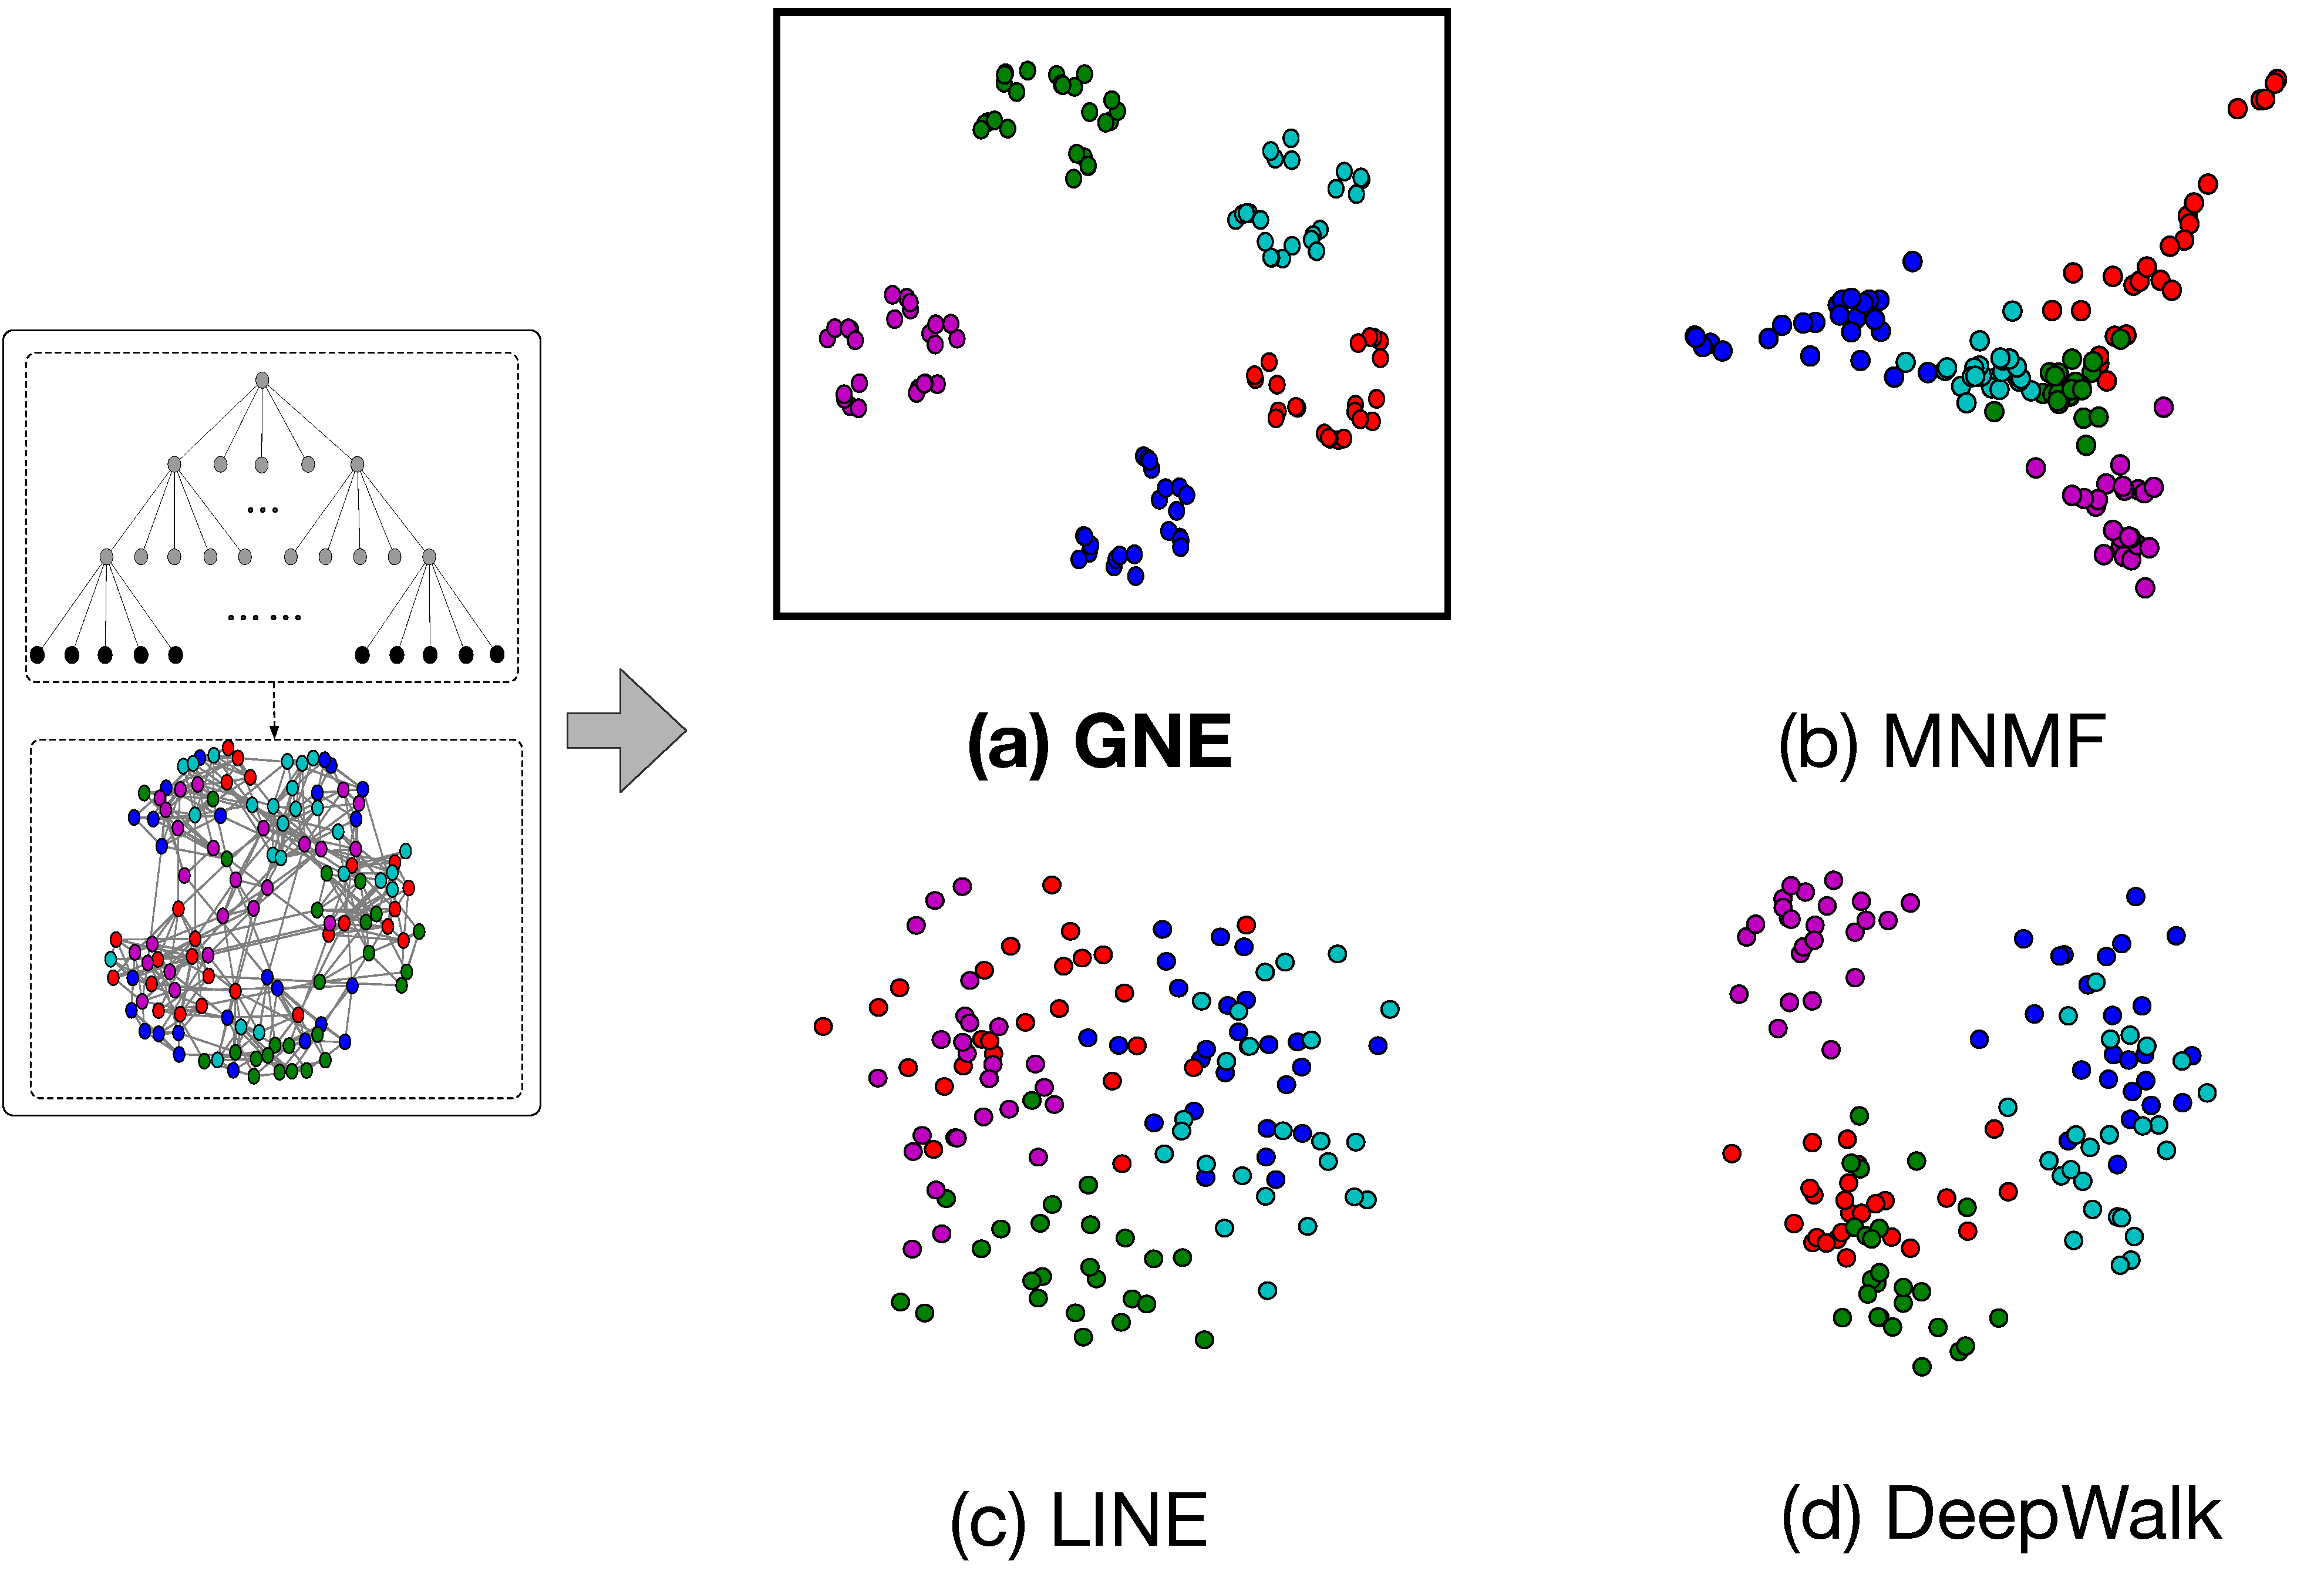
\includegraphics[width=0.45\textwidth]{figure/visualization.pdf}
		\caption{The visualization of node representations on different models}
		\label{fig:visualization}
	\end{figure}
	It can be seen from Fig.\ref{fig:visualization} that our model GNE embeds nodes on the different-scaled spherical surface hierarchically. It is evident that the node representations of GNE are consistent with modularity property at each hierarchy, i.e. higher intra-cluster similarity but lower inter-cluster similarity. That is to say, GNE integrally preserves the hierarchical community structure. Additionally, GNE has an outstanding performance on clustering nodes compared with others.
	
	

	\subsection{Node Classification}
	In order to verify the effectiveness of GNE on node classification, three real social networks with hierarchical community structure are used. The learned representations are used to classify the nodes into a set of labels. The classifier we used is Logistic Regression with sklearn package, and the evaluation metric is Accuracy. Different percentage of nodes are sampled randomly for evaluation, and the rest are for training. The results are averaged over 10 different runs. 

	Table \ref{tab:classification}. shows that GNE almost has a better performance than other models on different percentage of test data size. Since it's challengeable to extract the hierarchical clustering tree of big networks with the on-the-shelf works, for the networks of Georgeous University(9414nodes, 425639edges), our model uses the two-layer tree structure with the enrolment year as an indicator of data division, same with MNMF. In general, our model is robust no matter how much the percentage of test data accounts for, especifically on 10\% of the samples training, 90\% of the samples testing.
 
 	\section{Conclusion}
 	In this paper, we propose Galaxy Network Embedding (GNE) for network embedding to preserve the hierarchical community structure of a network. 
 	Specifically, we introduce an optimization problem with constraints and transform it into an unconstrained optimization problem more easily to be solved. Besides, we propose a spherical embedding method to maintain the hierarchical community structure from top to down. 
 	Empirically, we verify GNE in a variety of network datasets and applications. The extensive experimental results on vertex clustering and classification, as well as network visualization, demonstrate the advantages of GNE, especially on these networks with hierarchical community structure.

%% The file named.bst is a bibliography style file for BibTeX 0.99c
\bibliographystyle{named}
\bibliography{GNE}

\end{document}

